% Options for packages loaded elsewhere
\PassOptionsToPackage{unicode}{hyperref}
\PassOptionsToPackage{hyphens}{url}
\PassOptionsToPackage{dvipsnames,svgnames,x11names}{xcolor}
%
\documentclass[
  letterpaper,
  DIV=11,
  numbers=noendperiod]{scrartcl}

\usepackage{amsmath,amssymb}
\usepackage{iftex}
\ifPDFTeX
  \usepackage[T1]{fontenc}
  \usepackage[utf8]{inputenc}
  \usepackage{textcomp} % provide euro and other symbols
\else % if luatex or xetex
  \usepackage{unicode-math}
  \defaultfontfeatures{Scale=MatchLowercase}
  \defaultfontfeatures[\rmfamily]{Ligatures=TeX,Scale=1}
\fi
\usepackage{lmodern}
\ifPDFTeX\else  
    % xetex/luatex font selection
\fi
% Use upquote if available, for straight quotes in verbatim environments
\IfFileExists{upquote.sty}{\usepackage{upquote}}{}
\IfFileExists{microtype.sty}{% use microtype if available
  \usepackage[]{microtype}
  \UseMicrotypeSet[protrusion]{basicmath} % disable protrusion for tt fonts
}{}
\makeatletter
\@ifundefined{KOMAClassName}{% if non-KOMA class
  \IfFileExists{parskip.sty}{%
    \usepackage{parskip}
  }{% else
    \setlength{\parindent}{0pt}
    \setlength{\parskip}{6pt plus 2pt minus 1pt}}
}{% if KOMA class
  \KOMAoptions{parskip=half}}
\makeatother
\usepackage{xcolor}
\usepackage[margin=1in]{geometry}
\setlength{\emergencystretch}{3em} % prevent overfull lines
\setcounter{secnumdepth}{-\maxdimen} % remove section numbering
% Make \paragraph and \subparagraph free-standing
\makeatletter
\ifx\paragraph\undefined\else
  \let\oldparagraph\paragraph
  \renewcommand{\paragraph}{
    \@ifstar
      \xxxParagraphStar
      \xxxParagraphNoStar
  }
  \newcommand{\xxxParagraphStar}[1]{\oldparagraph*{#1}\mbox{}}
  \newcommand{\xxxParagraphNoStar}[1]{\oldparagraph{#1}\mbox{}}
\fi
\ifx\subparagraph\undefined\else
  \let\oldsubparagraph\subparagraph
  \renewcommand{\subparagraph}{
    \@ifstar
      \xxxSubParagraphStar
      \xxxSubParagraphNoStar
  }
  \newcommand{\xxxSubParagraphStar}[1]{\oldsubparagraph*{#1}\mbox{}}
  \newcommand{\xxxSubParagraphNoStar}[1]{\oldsubparagraph{#1}\mbox{}}
\fi
\makeatother


\providecommand{\tightlist}{%
  \setlength{\itemsep}{0pt}\setlength{\parskip}{0pt}}\usepackage{longtable,booktabs,array}
\usepackage{calc} % for calculating minipage widths
% Correct order of tables after \paragraph or \subparagraph
\usepackage{etoolbox}
\makeatletter
\patchcmd\longtable{\par}{\if@noskipsec\mbox{}\fi\par}{}{}
\makeatother
% Allow footnotes in longtable head/foot
\IfFileExists{footnotehyper.sty}{\usepackage{footnotehyper}}{\usepackage{footnote}}
\makesavenoteenv{longtable}
\usepackage{graphicx}
\makeatletter
\newsavebox\pandoc@box
\newcommand*\pandocbounded[1]{% scales image to fit in text height/width
  \sbox\pandoc@box{#1}%
  \Gscale@div\@tempa{\textheight}{\dimexpr\ht\pandoc@box+\dp\pandoc@box\relax}%
  \Gscale@div\@tempb{\linewidth}{\wd\pandoc@box}%
  \ifdim\@tempb\p@<\@tempa\p@\let\@tempa\@tempb\fi% select the smaller of both
  \ifdim\@tempa\p@<\p@\scalebox{\@tempa}{\usebox\pandoc@box}%
  \else\usebox{\pandoc@box}%
  \fi%
}
% Set default figure placement to htbp
\def\fps@figure{htbp}
\makeatother

\KOMAoption{captions}{tableheading}
\usepackage{float}          % For improved figure placement control (e.g., using [H])
\makeatletter
\renewcommand{\fps@figure}{H}
\usepackage{tabularx}        % For tables with automatic text wrapping
\newcolumntype{Y}{>{\centering\arraybackslash}X} % Custom column type for centered text
\usepackage{graphicx}        % For including images
\makeatletter
\@ifpackageloaded{caption}{}{\usepackage{caption}}
\AtBeginDocument{%
\ifdefined\contentsname
  \renewcommand*\contentsname{Table of contents}
\else
  \newcommand\contentsname{Table of contents}
\fi
\ifdefined\listfigurename
  \renewcommand*\listfigurename{List of Figures}
\else
  \newcommand\listfigurename{List of Figures}
\fi
\ifdefined\listtablename
  \renewcommand*\listtablename{List of Tables}
\else
  \newcommand\listtablename{List of Tables}
\fi
\ifdefined\figurename
  \renewcommand*\figurename{Figure}
\else
  \newcommand\figurename{Figure}
\fi
\ifdefined\tablename
  \renewcommand*\tablename{Table}
\else
  \newcommand\tablename{Table}
\fi
}
\@ifpackageloaded{float}{}{\usepackage{float}}
\floatstyle{ruled}
\@ifundefined{c@chapter}{\newfloat{codelisting}{h}{lop}}{\newfloat{codelisting}{h}{lop}[chapter]}
\floatname{codelisting}{Listing}
\newcommand*\listoflistings{\listof{codelisting}{List of Listings}}
\makeatother
\makeatletter
\makeatother
\makeatletter
\@ifpackageloaded{caption}{}{\usepackage{caption}}
\@ifpackageloaded{subcaption}{}{\usepackage{subcaption}}
\makeatother

\usepackage{bookmark}

\IfFileExists{xurl.sty}{\usepackage{xurl}}{} % add URL line breaks if available
\urlstyle{same} % disable monospaced font for URLs
\hypersetup{
  pdftitle={DATA221 Final Project},
  pdfauthor={Dariel Cruz Rodriguez; Yordi Hernandez},
  colorlinks=true,
  linkcolor={blue},
  filecolor={Maroon},
  citecolor={Blue},
  urlcolor={Blue},
  pdfcreator={LaTeX via pandoc}}


\title{DATA221 Final Project}
\author{Dariel Cruz Rodriguez \and Yordi Hernandez}
\date{}

\begin{document}
\maketitle


The goal of the project is to explore a number of datasets that may be
associated with political instability in the U.S. The data was taken
from the Seshat Databank under Creative Commons Attribution
Non-Commercial (CC By-NC SA) licensing.

\begin{center}\rule{0.5\linewidth}{0.5pt}\end{center}

\subsection{Data Wrangling}\label{data-wrangling}

\begin{itemize}
\tightlist
\item[$\boxtimes$]
  Read the (short) code book.
\item[$\boxtimes$]
  Numerical data need to be uploaded, interpolated, and properly saved.
  For the purpose of this project, interpolate each variable such that
  you obtain one point per year (within the range of available data).
\item[$\boxtimes$]
  Calculate (and then interpolate) the political instability index.
\item[$\boxtimes$]
  Display the DataFrame with all of the columns and the interpolated
  data for the years 1901-1910.
\end{itemize}

\begin{center}\rule{0.5\linewidth}{0.5pt}\end{center}

\phantomsection\label{timefilter-2}
\begin{longtable}[]{@{}lllllllllllllllll@{}}
\caption{The DataFrame with all of the columns and the interpolated data
for the years 1901-1910}\tabularnewline
\toprule\noalign{}
& time & polarization & ratio & assassination & executions &
insurrection & lynching & mass suicide & rampage & riot & terrorism &
war & total\_deaths & Height(cm) & EVI & HSUS \\
\midrule\noalign{}
\endfirsthead
\toprule\noalign{}
& time & polarization & ratio & assassination & executions &
insurrection & lynching & mass suicide & rampage & riot & terrorism &
war & total\_deaths & Height(cm) & EVI & HSUS \\
\midrule\noalign{}
\endhead
\bottomrule\noalign{}
\endlastfoot
0 & 1901 & 0.845472 & 0.651275 & 1.0 & 0.0 & 0.0 & 3.0 & 0.0 & 0.0 & 5.0
& 0.0 & 0.0 & 9.0 & 170.147403 & 1414.866130 & 30.663260 \\
1 & 1902 & 0.860217 & 0.645180 & 0.0 & 0.0 & 0.0 & 3.0 & 0.0 & 0.0 & 2.0
& 0.0 & 0.0 & 5.0 & 170.381602 & 1474.485794 & 31.272835 \\
2 & 1903 & 0.868912 & 0.639086 & 0.0 & 0.0 & 0.0 & 5.0 & 0.0 & 0.0 & 9.0
& 0.0 & 0.0 & 14.0 & 170.618785 & 1601.367749 & 31.312078 \\
3 & 1904 & 0.877794 & 0.627711 & 0.0 & 0.0 & 0.0 & 4.0 & 0.0 & 0.0 & 5.0
& 0.0 & 0.0 & 9.0 & 170.726188 & 1667.193907 & 31.879503 \\
4 & 1905 & 0.890111 & 0.606085 & 1.0 & 0.0 & 0.0 & 0.0 & 0.0 & 0.0 & 2.0
& 0.0 & 0.0 & 3.0 & 170.940995 & 1811.854852 & 32.514036 \\
5 & 1906 & 0.898414 & 0.596688 & 0.0 & 0.0 & 0.0 & 3.0 & 0.0 & 0.0 &
10.0 & 0.0 & 0.0 & 13.0 & 171.161172 & 1888.826416 & 33.091095 \\
6 & 1907 & 0.891646 & 0.607063 & 0.0 & 0.0 & 0.0 & 0.0 & 0.0 & 0.0 & 6.0
& 0.0 & 0.0 & 6.0 & 171.384034 & 1965.170701 & 33.132955 \\
7 & 1908 & 0.882256 & 0.610940 & 0.0 & 0.0 & 0.0 & 9.0 & 0.0 & 0.0 & 5.0
& 0.0 & 0.0 & 14.0 & 171.621216 & 2137.097683 & 33.724216 \\
8 & 1909 & 0.873668 & 0.608747 & 0.0 & 0.0 & 0.0 & 7.0 & 0.0 & 0.0 & 1.0
& 0.0 & 0.0 & 8.0 & 171.836023 & 2227.886274 & 34.314315 \\
9 & 1910 & 0.860964 & 0.602996 & 0.0 & 0.0 & 0.0 & 5.0 & 0.0 & 0.0 &
19.0 & 1.0 & 0.0 & 25.0 & 172.080664 & 2325.601346 & 34.346872 \\
\end{longtable}

We decided against using only years 1901-1910, because it would be too
short of a time frame to analyze and the data would be limited to train
on. Instead, we opted to use the time period between 1815 - 1968,
because all of the years in between contain data for all of the
variables with the exception of one year that had a missing ratio value,
which we will interpolate by taking the average of the two years
surrounding it. We feel that analyzing the years 1815 - 1968, an entire
century and more, will give us a better understanding of the data and
allow us to train our model more effectively to account for generational
shifts in political instability.

\subsection{Exploratory Data Analysis}\label{exploratory-data-analysis}

\begin{itemize}
\tightlist
\item[$\boxtimes$]
  Conduct an exploratory data analysis
\item[$\boxtimes$]
  Summarize your main findings (most interesting/insightful conclusions)
  in a short paragraph and include appropriate visualizations.
\end{itemize}

\begin{center}\rule{0.5\linewidth}{0.5pt}\end{center}

\begin{figure}

{\centering \pandocbounded{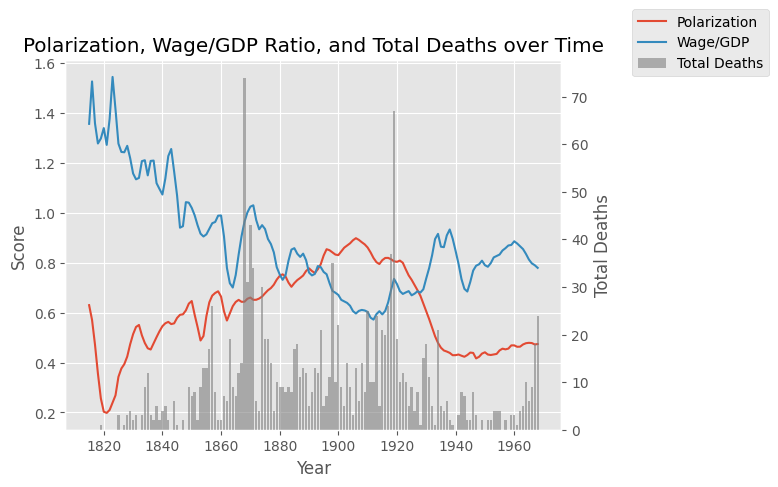
\includegraphics[keepaspectratio]{FInal_project_files/figure-pdf/different-graphs1-output-1.png}}

}

\caption{Line graph/bar plot showing the relationship between
Polarization \& Wage/GDP over time and total deaths}

\end{figure}%

\begin{figure}

{\centering \pandocbounded{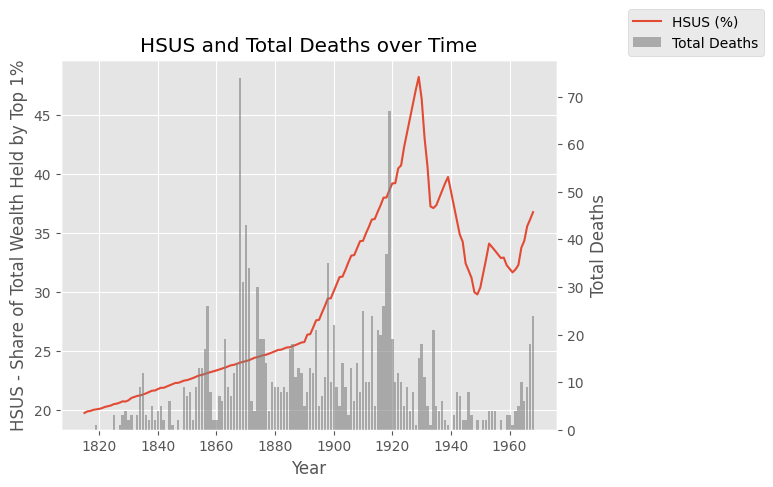
\includegraphics[keepaspectratio]{FInal_project_files/figure-pdf/different-graphs2-output-1.png}}

}

\caption{Line graph/bar plot showing the relationship between HSUS over
time and total deaths}

\end{figure}%

\begin{figure}

{\centering \pandocbounded{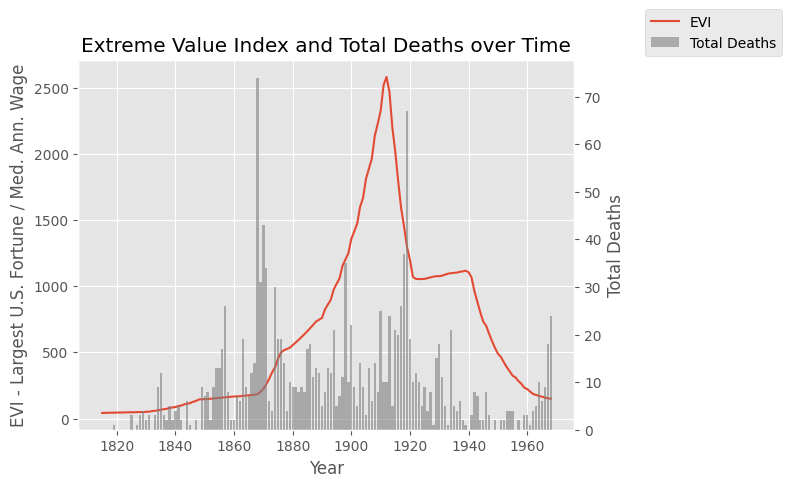
\includegraphics[keepaspectratio]{FInal_project_files/figure-pdf/different-graphs3-output-1.png}}

}

\caption{Line graph/bar plot showing the relationship between EVI over
time and total deaths}

\end{figure}%

\begin{figure}

{\centering \pandocbounded{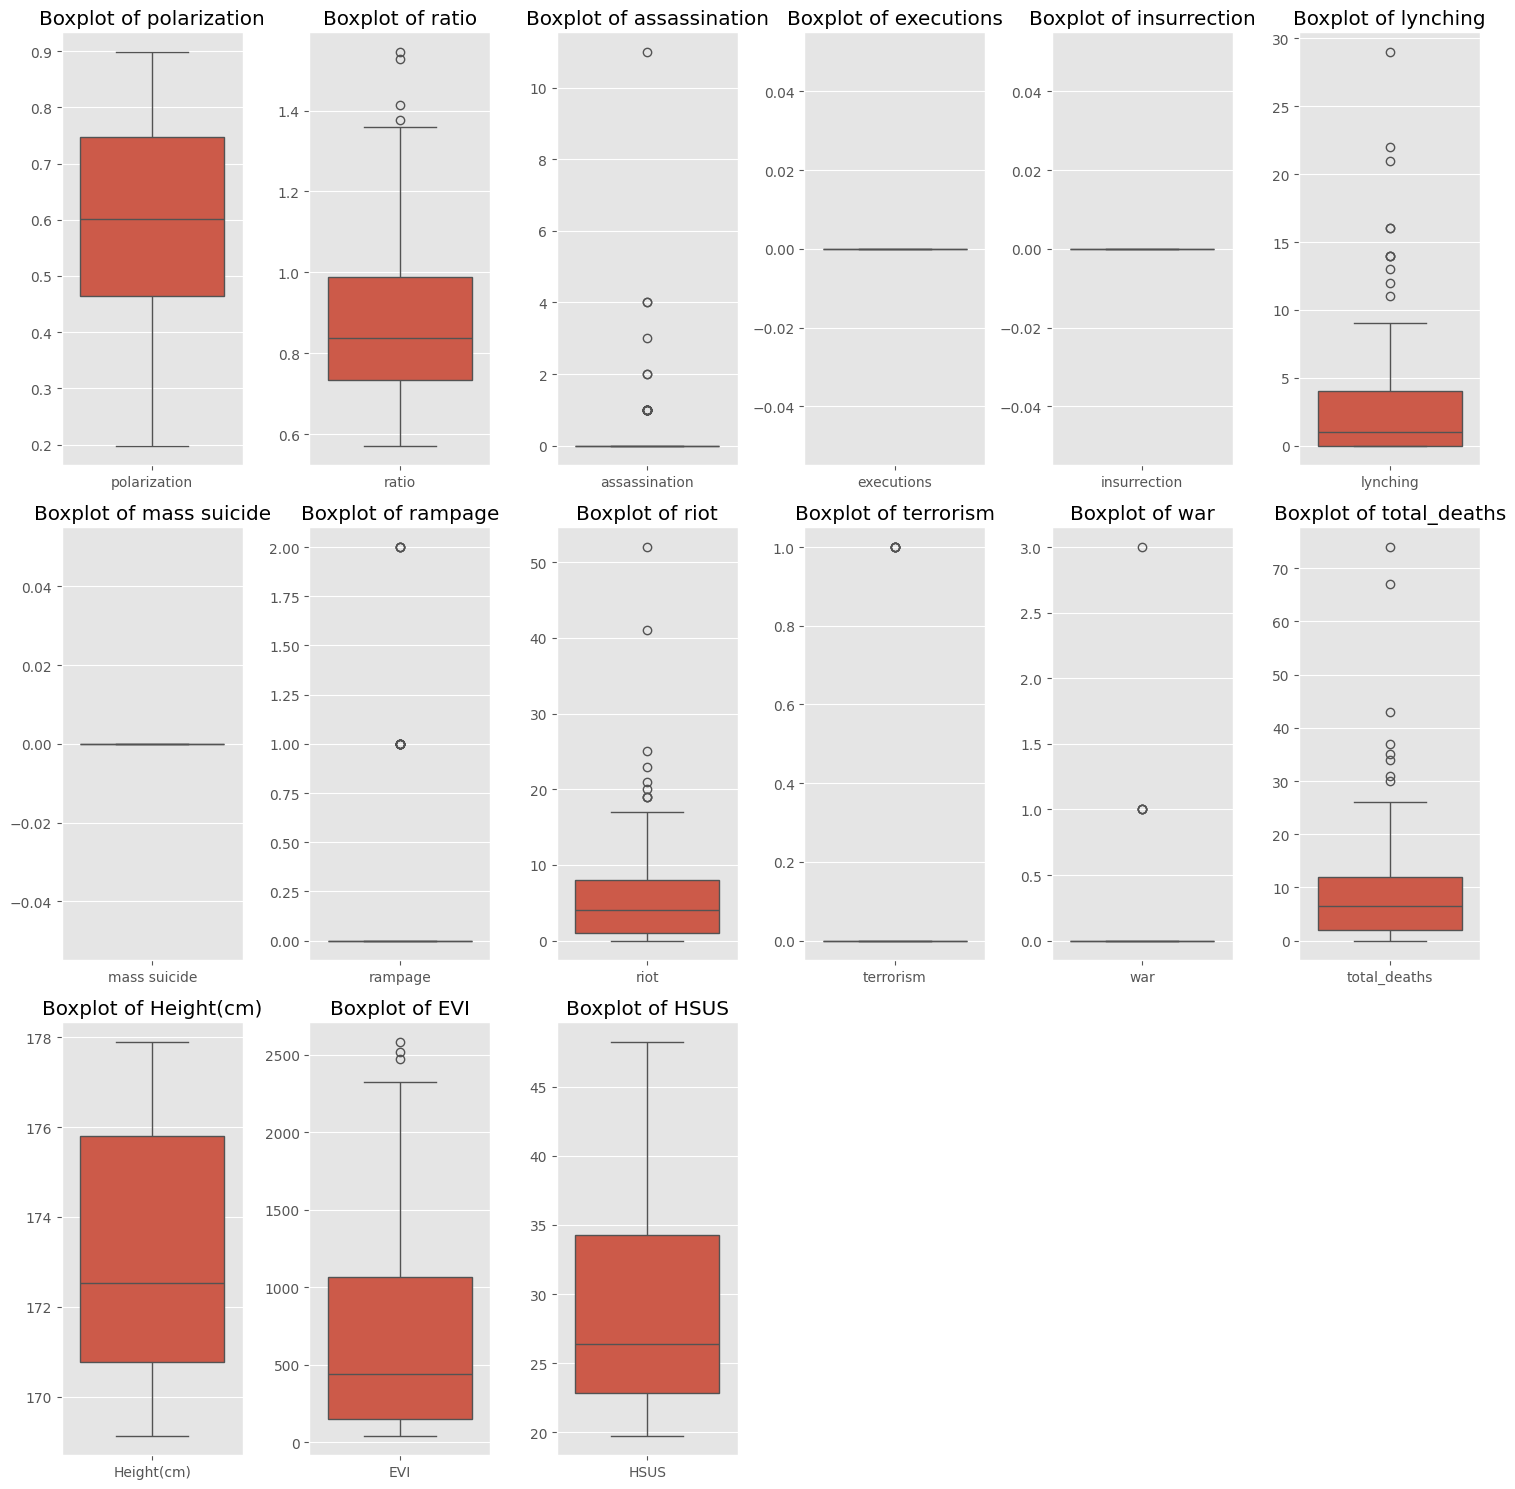
\includegraphics[keepaspectratio]{FInal_project_files/figure-pdf/boxplots-variables-output-1.png}}

}

\caption{Boxplots showing the distribution of each variable in the
dataset}

\end{figure}%

\begin{figure}

{\centering \pandocbounded{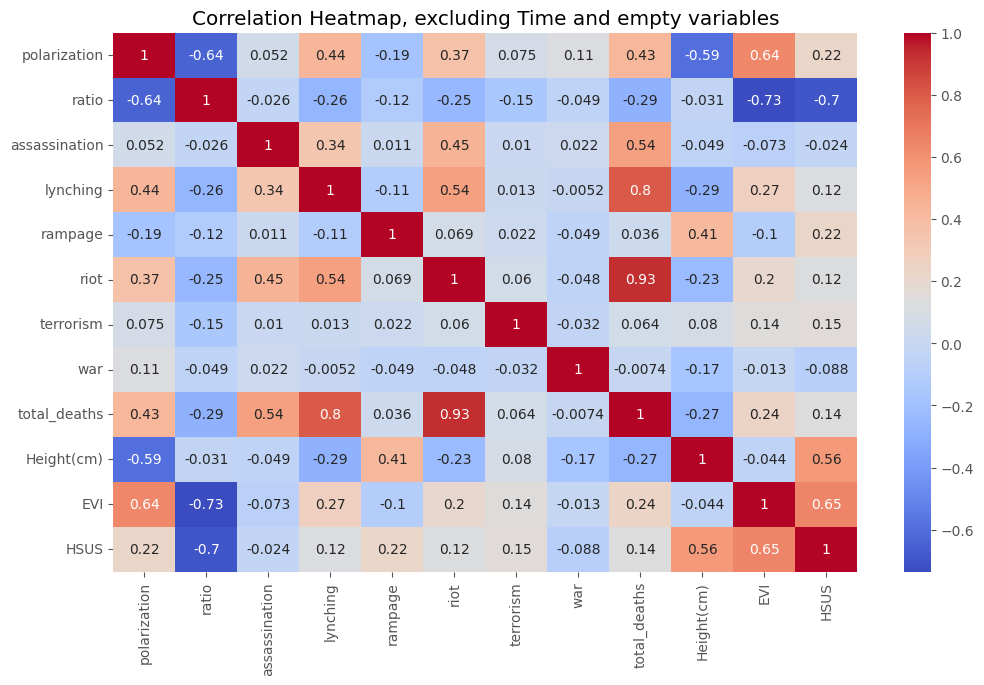
\includegraphics[keepaspectratio]{FInal_project_files/figure-pdf/correlation-heatmap-output-1.png}}

}

\caption{Correlation heatmap showing the relationship between each
variable in the dataset, excluding Time and empty variables}

\end{figure}%

After conducting an exploratory data analysis, we have come to several
conclusions.

Firstly, within the subset of the years 1815 and 1968 that we selected
for our analysis, political instability remained relatively stable over
the years, in fact actually decreasing as 1968 approached. In addiiton,
political instability appears visually to be inverse (or negatively
correlated) to the Wage/GDP ratio. This is interesting because it
suggests that as the wage/GDP ratio increases, political instability
decreases. Another way to describe this could be that as wages increase,
political instability generally decreases. This can be verified
mathematically as well, as the correlation coefficient between the ratio
and polarization is \(-0.64\), which represents a strong negative
correlation.

Additionally within the correlation table, the wage/GDP ratio is also
strongly negatively correlated with the Extreme Value Index and HSUS
which is entirely reasonable because both metrics represent larger
values for more wealth disparity and smaller values for wealth equality
while the ratio is higher for wealth equality and smaller for wealth
disparity, the complete opposite.

Another interesting finding is how strongly the variable Height(cm) is
correlated with multiple metrics in the dataset. Height is negatively
correlated with polarization at a value of \(-0.59\) and with HSUS at a
value of \(0.56\), suggesting that as height increases, polarization
decreases. I do not believe this is causation however, because at the
same time height is positively correlated with time at a value of
\(0.64\), leading me to believe that height can be construed as another
measure for time. As time goes on, people got taller on average but
coincidentally at the same time political instability went down.

The only apparent trend I could identify visually is the similar bumps
and increase in both HSUS and EVI metrics at the same time, presumably
because they measure similar things.

There are 154 entries in our dataset, which could lead to a lot of noise
later on when we build our models. This is accompanied as well by
several outliers in the individual types of deaths that occured in each
year and a few outliers with ratio and EVI. To account for this, we may
need to consider reducing the number of features we consider in our
dataset. Specifically, I would consider dropping time and total\_deaths,
because they are directly linked to other variables in the set.

\subsection{Find the best regressor}\label{find-the-best-regressor}

Find the best regressor that would predict the instability index from
the various predictors. To be clear, you are asked to compare a limited
set of regressors of your choice -- not to identify the theoretically
optimal one.

\begin{itemize}
\tightlist
\item[$\boxtimes$]
  Explain your modeling choices.
\item[$\boxtimes$]
  Interpret any evaluation metrics you use.
\item[$\boxtimes$]
  Summarize your conclusions in a short paragraph, i.e., the most
  interesting conclusion(s), the model that produced it, and how the
  model was chosen. You may include a figure if you find it helpful.
\end{itemize}

\begin{center}\rule{0.5\linewidth}{0.5pt}\end{center}

\phantomsection\label{best-regressor}
\begin{longtable}[]{@{}llll@{}}
\caption{R2, MSE, and MAE scores aross multiple regression
models}\tabularnewline
\toprule\noalign{}
& R2 & MSE & MAE \\
\midrule\noalign{}
\endfirsthead
\toprule\noalign{}
& R2 & MSE & MAE \\
\midrule\noalign{}
\endhead
\bottomrule\noalign{}
\endlastfoot
Linear Regression & 1.000000 & 8.981265e-29 & 7.918016e-15 \\
Ridge Regression & 0.999942 & 4.836788e-03 & 5.563760e-02 \\
Lasso Regression & 0.996825 & 2.632591e-01 & 2.519983e-01 \\
Random Forest & 0.942836 & 4.739526e+00 & 1.332553e+00 \\
\end{longtable}

After choosing 4 of the most used regressors (Linear, Ridge, Lasso, and
Random Forest classifier), the models were trained and tested in order
to compare which one performed the best. The metrics used in order to
compare performance were R², which explains variance, MSE, which
penalizes larger errors heavily, so the lower score the better, and MAE,
where the lower the score the better.

Based on the results, Linear Regression performed the best as it had the
highest R², lowest mean squared error, and mean absolute error. The
performance was nearly perfect since it explained nearly 100 percent of
the variance in the instability index with little error. Because Linear
Regression achieved such great results, complex models like Random
Forest were not necessary. Ridge and Lasso models performed well, yet
provided no advantage, confirming that feature redundancy and
multicollinearity were not concerns.

Additionally, the regressors were tested with a smaller subset
containing only 10 years, which yielded similar results. Linear
Regression was still the best performer.

\begin{figure}

{\centering \pandocbounded{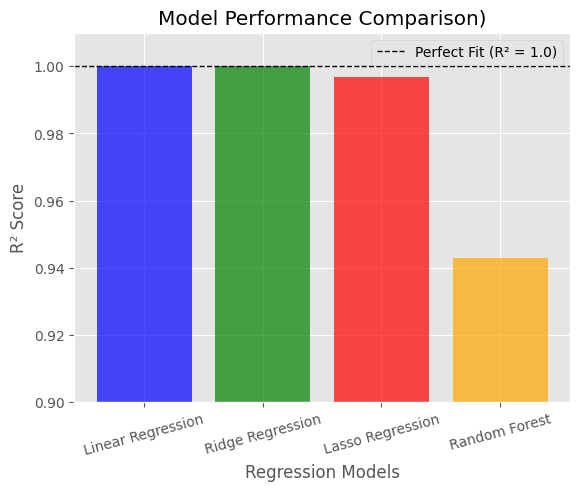
\includegraphics[keepaspectratio]{FInal_project_files/figure-pdf/model-performance-comparison-output-1.png}}

}

\caption{R2 scores for each regression model}

\end{figure}%

\subsection{Find the best dimensionality reduction for
regression}\label{find-the-best-dimensionality-reduction-for-regression}

You can restrict this part to reducing the data to two dimensions, to
three dimensions, or explore both options. You can test your variables
using the best regressor found in the previous section or a small number
of regressors (2-3 models at most).

\begin{itemize}
\tightlist
\item[$\boxtimes$]
  Explain modeling choices and evaluation metrics.
\item[$\boxtimes$]
  Summarize your conclusions in a short paragraph, i.e., the most
  interesting conclusion(s), the model that produced it, and how the
  model was chosen. You may include a figure if you find it helpful
\end{itemize}

\begin{center}\rule{0.5\linewidth}{0.5pt}\end{center}

\phantomsection\label{best-dimensionality-reduction}
\begin{longtable}[]{@{}lllll@{}}
\caption{R2, MSE, and MAE scores for each dimensionality reduction
method}\tabularnewline
\toprule\noalign{}
& Reduction Method & R2 Score & MSE & MAE \\
\midrule\noalign{}
\endfirsthead
\toprule\noalign{}
& Reduction Method & R2 Score & MSE & MAE \\
\midrule\noalign{}
\endhead
\bottomrule\noalign{}
\endlastfoot
0 & PCA (2D) & 0.355357 & 53.448476 & 5.832352 \\
1 & PCA (3D) & 0.922641 & 6.413987 & 1.957521 \\
2 & Feature Selection (Top 2) & 0.989286 & 0.888305 & 0.596215 \\
3 & Feature Selection (Top 3) & 0.994036 & 0.494466 & 0.405268 \\
\end{longtable}

\begin{figure}

{\centering \pandocbounded{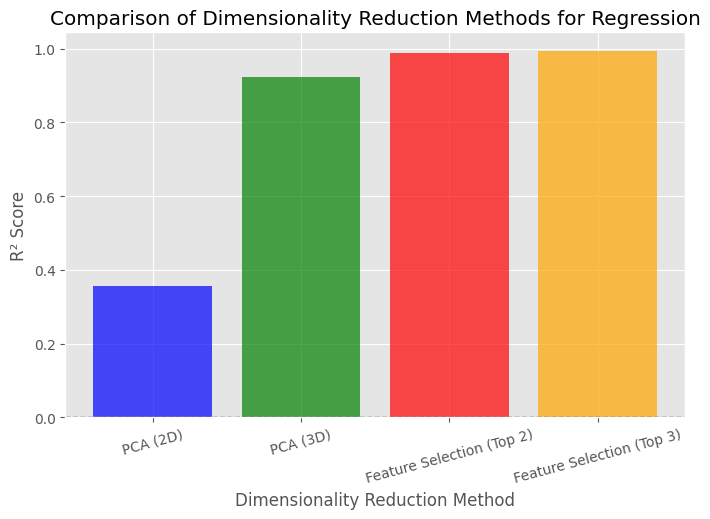
\includegraphics[keepaspectratio]{FInal_project_files/figure-pdf/comparison-dimensionalityreductionmethods-regression-output-1.png}}

}

\caption{R2 scores for each dimensionality reduction method}

\end{figure}%

\begin{verbatim}
9.37 + (1.08 * assassination) + (4.49 * lynching) + (7.24 * riot) 
\end{verbatim}

\begin{figure}

{\centering \pandocbounded{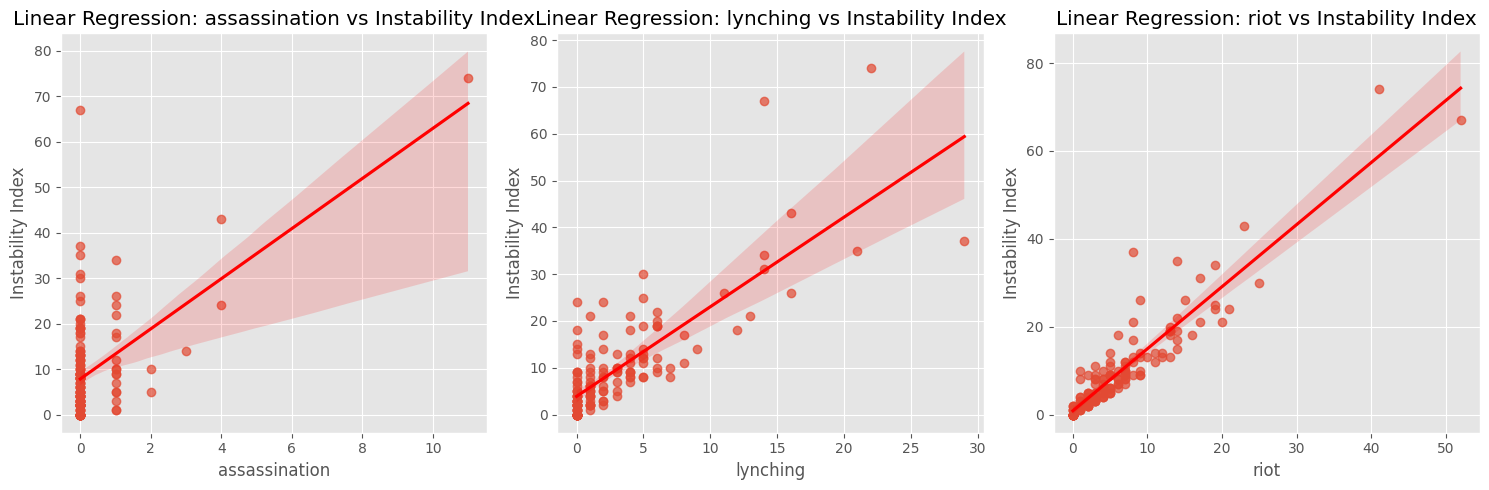
\includegraphics[keepaspectratio]{FInal_project_files/figure-pdf/linear-regression-output-2.png}}

}

\caption{Linear regression model with selected features}

\end{figure}%

\begin{figure}

{\centering \pandocbounded{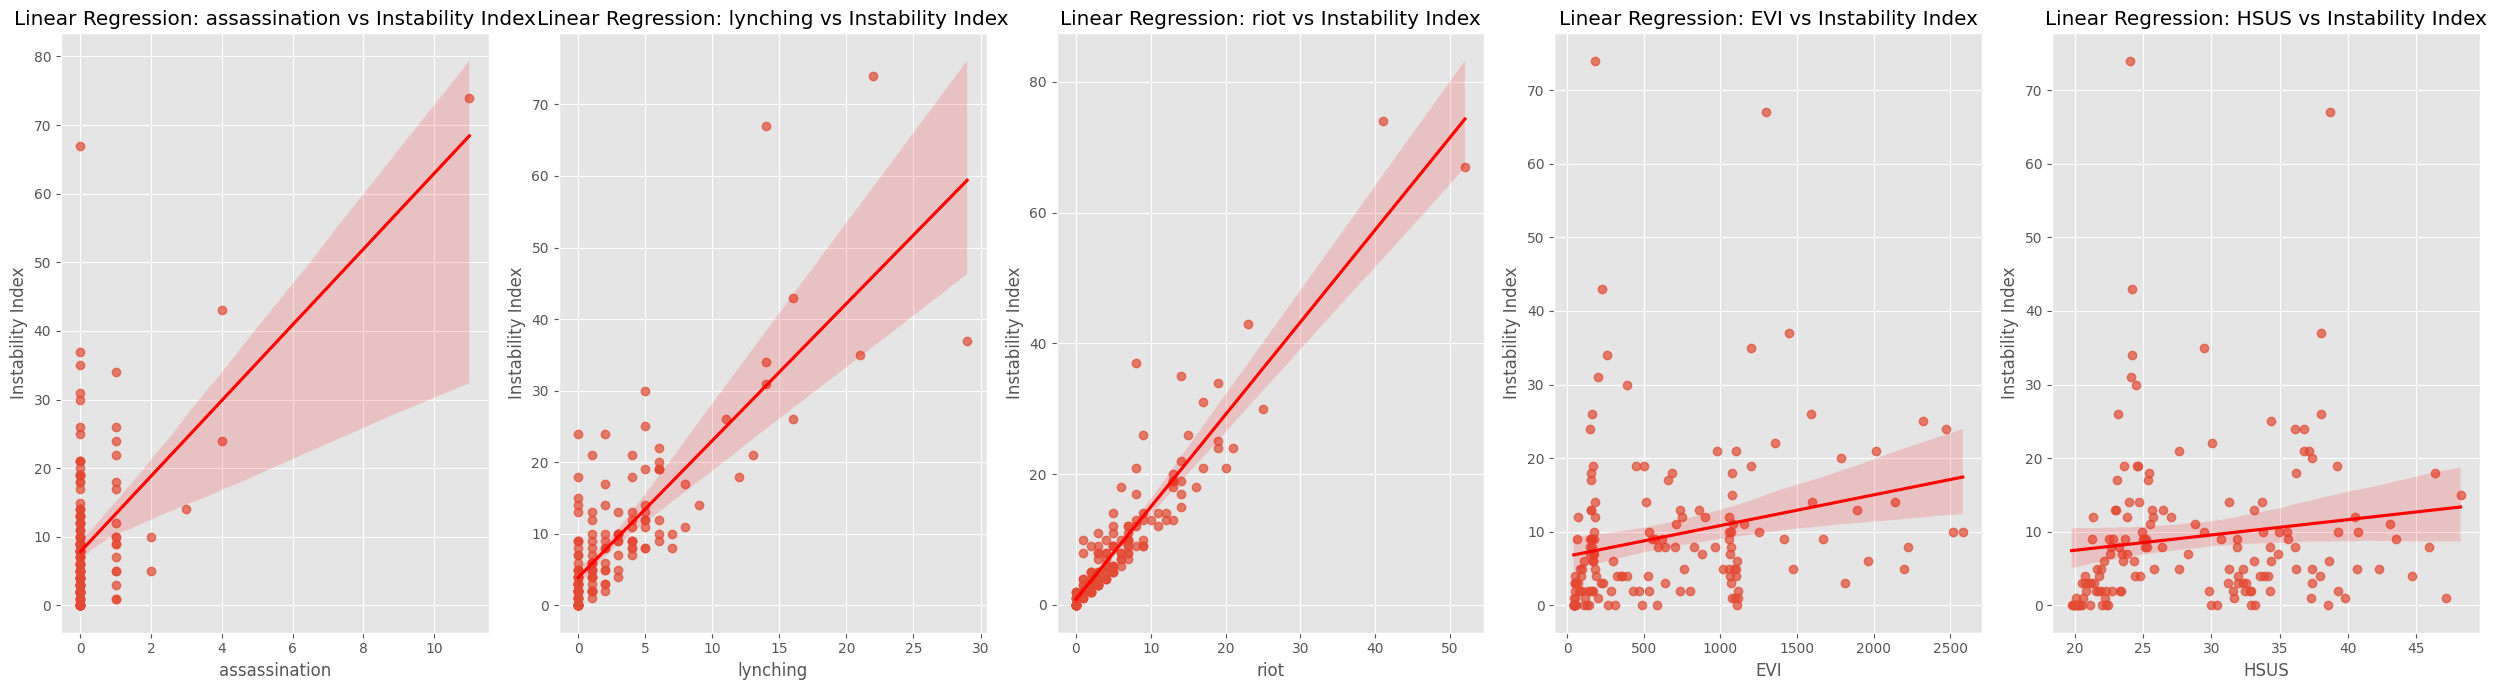
\includegraphics[keepaspectratio]{FInal_project_files/figure-pdf/linear-regression-extended-output-1.png}}

}

\caption{Linear regression model with additional selected features (EVI,
HSUS)}

\end{figure}%

\begin{figure}

{\centering \pandocbounded{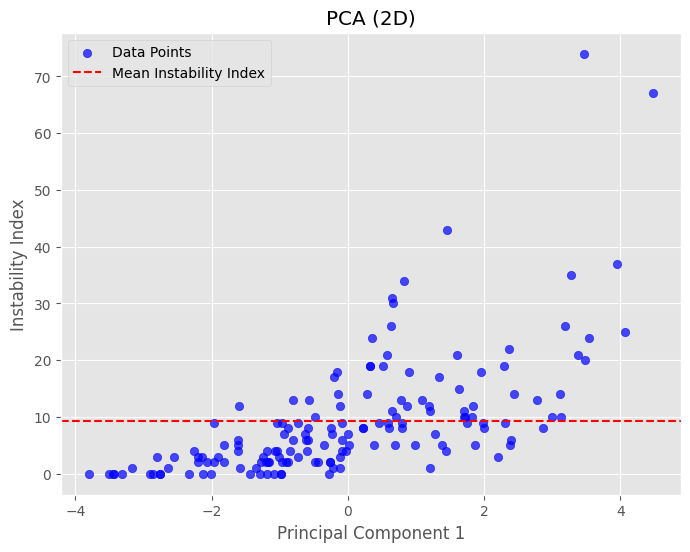
\includegraphics[keepaspectratio]{FInal_project_files/figure-pdf/pca-2d-plot-output-1.png}}

}

\caption{PCA plot in 2D}

\end{figure}%

In order to compare dimensionality the choices used were PCA which it's
purpose was to capture the most variance in the data.

Feature selection was also implemented. The purpose of feature selection
is to retain the most relevant predictors based on significance.
Similarly to the problem above, R2 score, MSE, and MAE were used as
metrics.

After executing the model, Feature selection with 3 features performed
the best suggesting keeping the main predictors yields better results.
On the other hand PCA performed poorly suggesting that important data is
lost when performing the model. Based on the results it is safe to say
Linear regression with selected features is the best option as it
provides both interpretability and superior regression performance.

\subsection{Find the best dimensionality reduction for unsupervised
classification}\label{find-the-best-dimensionality-reduction-for-unsupervised-classification}

Use only the predictor columns and not the outcome (instability) for
classification. You can restrict this part to reducing the data to two
dimensions, to three dimensions, or explore both options.

\begin{itemize}
\tightlist
\item[$\boxtimes$]
  You can test your variables using k-means or a small number of
  classifiers (2-3 models at most).
\item[$\boxtimes$]
  Explain modeling choices and evaluation metrics.
\item[$\boxtimes$]
  Summarize your conclusions in a short paragraph, i.e., the most
  interesting conclusion(s), the model that produced it, and how the
  model was chosen. You may include a figure if you find it helpful.
\end{itemize}

\begin{center}\rule{0.5\linewidth}{0.5pt}\end{center}

\begin{figure}

{\centering \pandocbounded{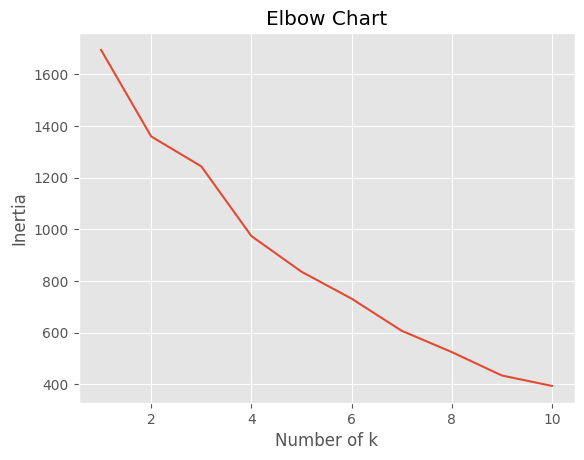
\includegraphics[keepaspectratio]{FInal_project_files/figure-pdf/kmeans-elbow-output-1.png}}

}

\caption{Elbow chart to determine the optimal number of clusters for
KMeans}

\end{figure}%

\begin{figure}

{\centering \pandocbounded{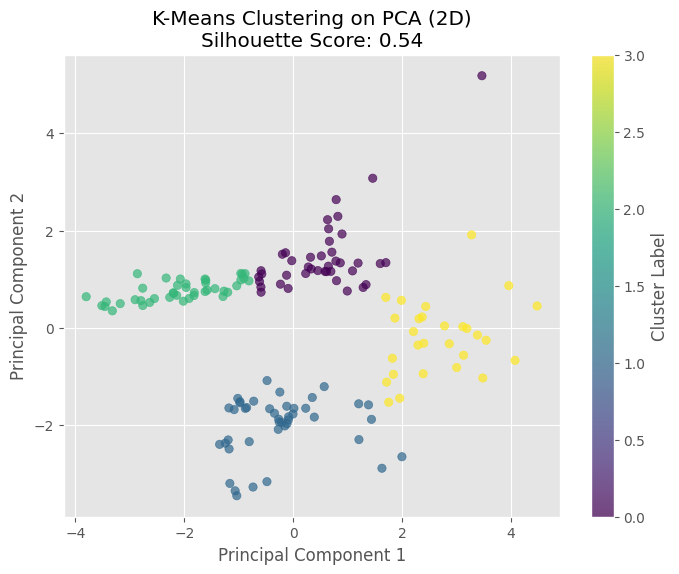
\includegraphics[keepaspectratio]{FInal_project_files/figure-pdf/kmeans-clustering-output-1.png}}

}

\caption{K-Means clustering on PCA (2D)}

\end{figure}%

\begin{figure}

{\centering \pandocbounded{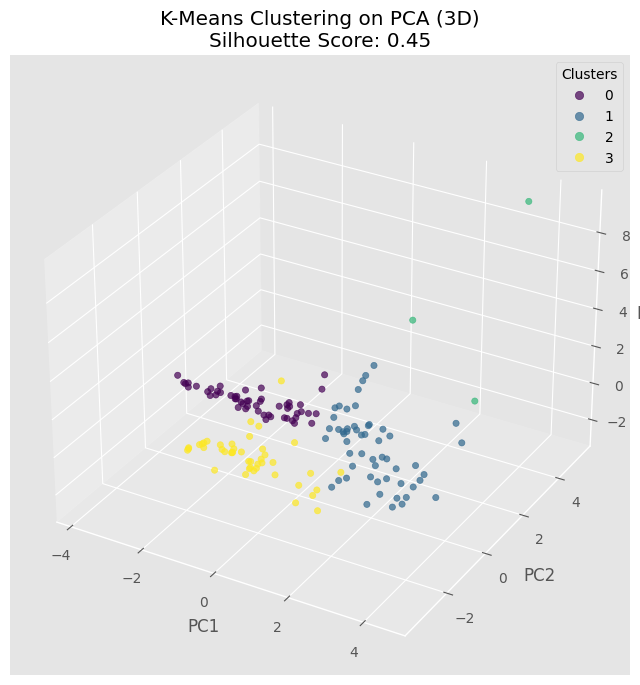
\includegraphics[keepaspectratio]{FInal_project_files/figure-pdf/kmeans-clustering2-output-1.png}}

}

\caption{K-Means clustering on PCA (3D)}

\end{figure}%

We applied PCA to reduce the predictor data into lower dimensions (2D
and 3D) so that the structure of the data can be visualized and
processed. K-Means clustering was the chosen model to classify the data
based on the reduced dimensions because it's suitable for continuous,
numeric data like the ratios and scores in our dataset. (Figure 12 and
Figure 13)

To determine the optimal number of clusters we evaluated multiple
K-values using the Elbow method (Figure 11) and then confirming our
selected K-value by comparing the Silhoutte score (Figure 12 and Figure
13, figure title). The elbow method is a visual tool to determine at
what value \emph{k} intertia begins to level off, another way to
represent the point where adding more clusters produces diminishing
returns. The silhoutte score measures how well-distinct and compact
clusters are by measure the relative distance to eachother within the
cluster. Using both of these metrics allowed us to select a k value that
did not have high interia and too few clusters, while also avoiding the
opposite issue of having too many clusters and overfitting our data.

Our findings showed that reducing the data to 2D and 3D dimensions using
PCA produced moderate separation amongst the clusters (which was the
best result we could achieve). The K-Means model with 4 clusters was the
best performer, as it produced the highest Silhoutte score and the most
distinct clusters. This suggests that the data can be classified into 4
distinct groups based on the reduced dimensions. Despite this, whether
it be due to the data itself or otherwise, the clusters still show some
overlap at the boundaries and aren't as distinct as we'd have liked.
(Figure 12, green and purple clusters)

\subsection{Briefly explore the clusters of instability
scores}\label{briefly-explore-the-clusters-of-instability-scores}

Consider the cluster labels from the best clustering scheme from
previous section or from clustering using all/most of the original
features. Apply it to the corresponding records of the outcome column
(instability).

\begin{itemize}
\tightlist
\item[$\boxtimes$]
  Create a visualization of the results.
\item[$\boxtimes$]
  Summarize your conclusions. To be clear, the summary can be very
  short, and may be that the clusters do not exhibit any discernable or
  interpretable pattern. You may include a figure if you find it
  helpful.
\end{itemize}

\begin{center}\rule{0.5\linewidth}{0.5pt}\end{center}

\begin{figure}

{\centering \pandocbounded{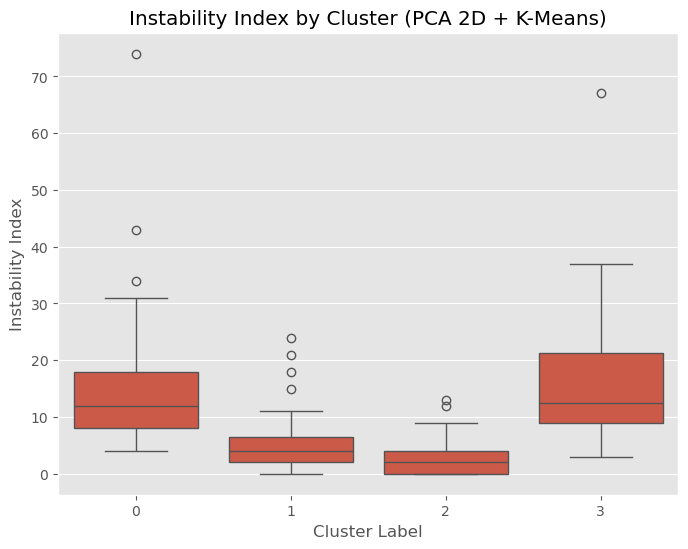
\includegraphics[keepaspectratio]{FInal_project_files/figure-pdf/instability-index-clustering-output-1.png}}

}

\caption{Instability index distribution by cluster}

\end{figure}%

\begin{figure}

{\centering \pandocbounded{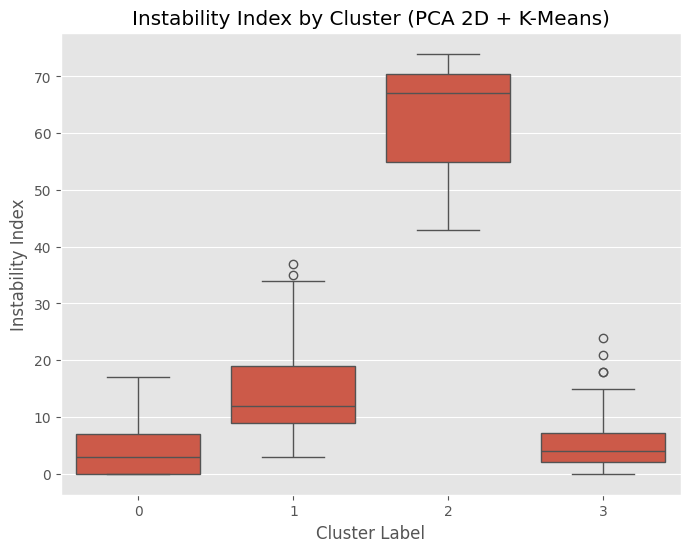
\includegraphics[keepaspectratio]{FInal_project_files/figure-pdf/instability-index-clustering3d-output-1.png}}

}

\caption{Instability index distribution by cluster}

\end{figure}%

Each cluster exhibits a different median Instability Index--- Clusters 1
and 2 show lower medians between 5 and 6 while Clusters 0 and 3 show
higher medians between the values 10-15. (Figure 14)

There is a notable overlap amongst the distributions of all the
clusters, suggesting that the clusters may not be well defined. Overall,
while ther eare some differences in central tendencies, the clusters
don't separate cleanly by Instability Index and there is not a clear,
discernable, and interpretable pattern that is useful for our analysis.

In the PCA 3D model with K-Means clusteirng, the distribution of cluster
2 is more spread out and pronounced than the other clusters, with no
overlap. The other clusters however, still have significant overlap and
are not as distinct. The data does not separate cleanly by instability
index, suggesting that instability is not the only factor impacting our
parameters. (Figure 15)

\subsection{Consider a real life modeling/prediction
problem}\label{consider-a-real-life-modelingprediction-problem}

\begin{itemize}
\tightlist
\item[$\boxtimes$]
  Try a large number (100? 1000?) different models
\item[$\boxtimes$]
  Examine their performances
\item[$\boxtimes$]
  Select the one that scores best on your performance metric of choice
\item[$\boxtimes$]
  Briefly discuss the potential disadvantage (or potential danger) of
  such and approach and how you might go about mitigating it.
\end{itemize}

\begin{center}\rule{0.5\linewidth}{0.5pt}\end{center}

\phantomsection\label{model-performance-table}
\begin{longtable}[]{@{}llll@{}}
\caption{MSE and R2 scores for each regression model averaged over 100
epochs}\tabularnewline
\toprule\noalign{}
& Model & MSE & R2 Score \\
\midrule\noalign{}
\endfirsthead
\toprule\noalign{}
& Model & MSE & R2 Score \\
\midrule\noalign{}
\endhead
\bottomrule\noalign{}
\endlastfoot
5 & Gradient Boosting & 36.492536 & 0.578757 \\
4 & Random Forest & 45.321113 & 0.476846 \\
0 & Linear Regression & 55.276529 & 0.361928 \\
2 & Lasso Regression & 55.578276 & 0.358445 \\
1 & Ridge Regression & 56.965077 & 0.342437 \\
3 & Decision Tree & 168.892049 & -0.949566 \\
\end{longtable}

\begin{figure}

{\centering \pandocbounded{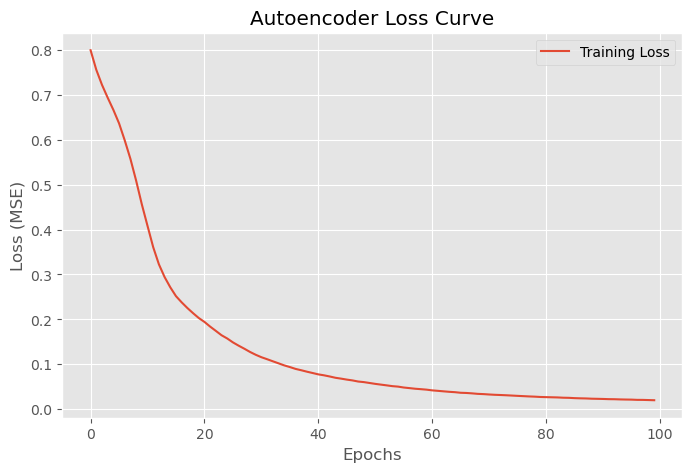
\includegraphics[keepaspectratio]{FInal_project_files/figure-pdf/autoencoder-loss-curve-output-1.png}}

}

\caption{Training loss curve for the autoencoder model}

\end{figure}%

\begin{figure}

{\centering \pandocbounded{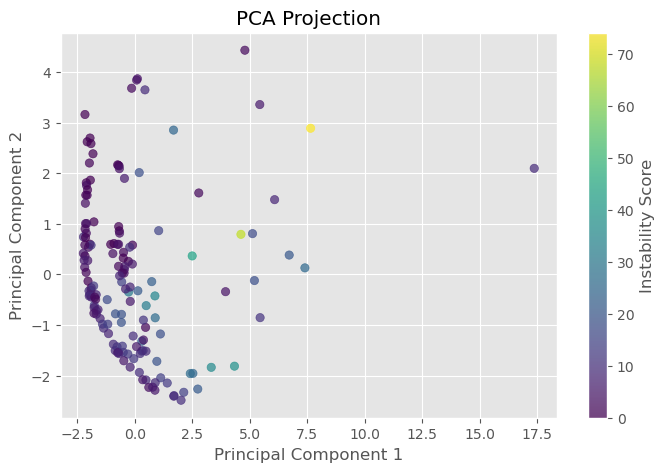
\includegraphics[keepaspectratio]{FInal_project_files/figure-pdf/pca-projection-model-performance-output-1.png}}

}

\caption{PCA projection of the latent space colored by Instability
Score}

\end{figure}%

The results show that linear models (Linear Regression, Ridge, Lasso)
performed best, with near-perfect R² scores, suggesting a strong linear
relationship in the data---but also raising concerns about overfitting
or data leakage. Tree-based models (Random Forest, Decision Trees,
Gradient Boosting) had mixed performance, sometimes scoring well but
also showing high error and instability, likely due to sensitivity to
hyperparameters or feature selection issues. (Table 4)

The wide range of results highlights the risk of blindly testing a large
number of models (100-1000) without proper validation. Some models
perform well by chance rather than true predictive power. To mitigate
overfitting and instability, cross-validation, hyperparameter tuning,
and feature selection are crucial. While testing many models helps
identify strong candidates, efficient selection and proper validation
matter more than force experimentation like training 100 models.

Using an autoencoder for this part was helpful since it reduced the
high-dimensional feature space into a more compact representation,
helping models focus on the most relevant patterns rather than redundant
data. It also reduced time consumption by compressing the data in an
optimal way. The Training Loss gradually decreases over epochs and does
not decrease significantly at the start of the model, which is what we
want to see to avoid overfitting on the training data. (Figure 16)

\subsection{Conclusion}\label{conclusion}

In conclusion, our analysis covered political instability over 150 years
and handled missing values through linear interpolation.

In our exploratory data anlysis, we identified a strong negative
correlation between the Wage/GDP ratio and political instability
suggesting that increasing wages may coincide with lower instability.
There were other interesting correlations like the inverse between
Height and polarization scores, but they more likely than not reflected
individual trends than causation.

When building regression models, Linear Regression achieved near-perfect
performance across multiple metrics, highlighting that there is a linear
relationship within the data. Ridge and Lasso also did well, but more
complex models didn't add much to the performance and had marginal
improvement at best, like Random Forest. This lesson highlights the
importance of proper model selection, especially because the more
complex models were more prone to overfitting and instability as a
result of noise in the data, while simpler models were more robust and
less prone to capturing noise.

Considering dimensionality reduction, Feature Section with 3 features
performed significantly well compared to PCA-based methods because they
retained the most relevant predictors and were more interpretable. PCA
in 3D provided moderate results, but the loss of important data was a
concern and made it less effective than targetting the most relevant
predictors. This highlighted the importance of feature selection and the
pitfalls of dimensionality reduction without considering the context of
the data.

Lastly, in our unsupervised classification section, we applied PCA with
K-Means clustering, as reccomended in the project instructions, to
classify the data into 4 clusters. We chose \(k=4\) by using the Elbow
method and Silhoutte score to find the optimal number of clusters that
would not overfit the data but also wouldn't underfit it. (a happy
medium, as you say) Although \(k=4\) clusters was the best for 3D and 2D
PCA with K-Means, some overlap continued to show limiting clear
separation between clusters on the account of instability index alone.

In the final moeling considerations section, we tested 6 models 100
times, aggregated multiple evaluation metrics, and found that testing a
large number of models at a time can lead to overfitting and at worst,
misleading results. More cross-validation and hyperparameter tuning are
preferred to blindly testing a large number of models if model
reliability is our priority.




\end{document}
